\subsection{Non-linear decision boundaries}

Next, we're considering non-linear separation, where our dataset can't be separated by a linear hyperplane, but by some other non-linear decision boundary. Consider the example in \ref{fig:5_not_linear_separable}. Our idea to solve this separation is to \textbf{lift the number of dimensions}\sidenote{Lift number of dimensions}.

\begin{figure}[H]
  \centering
  \begin{subfigure}{\textwidth}
    \centering
    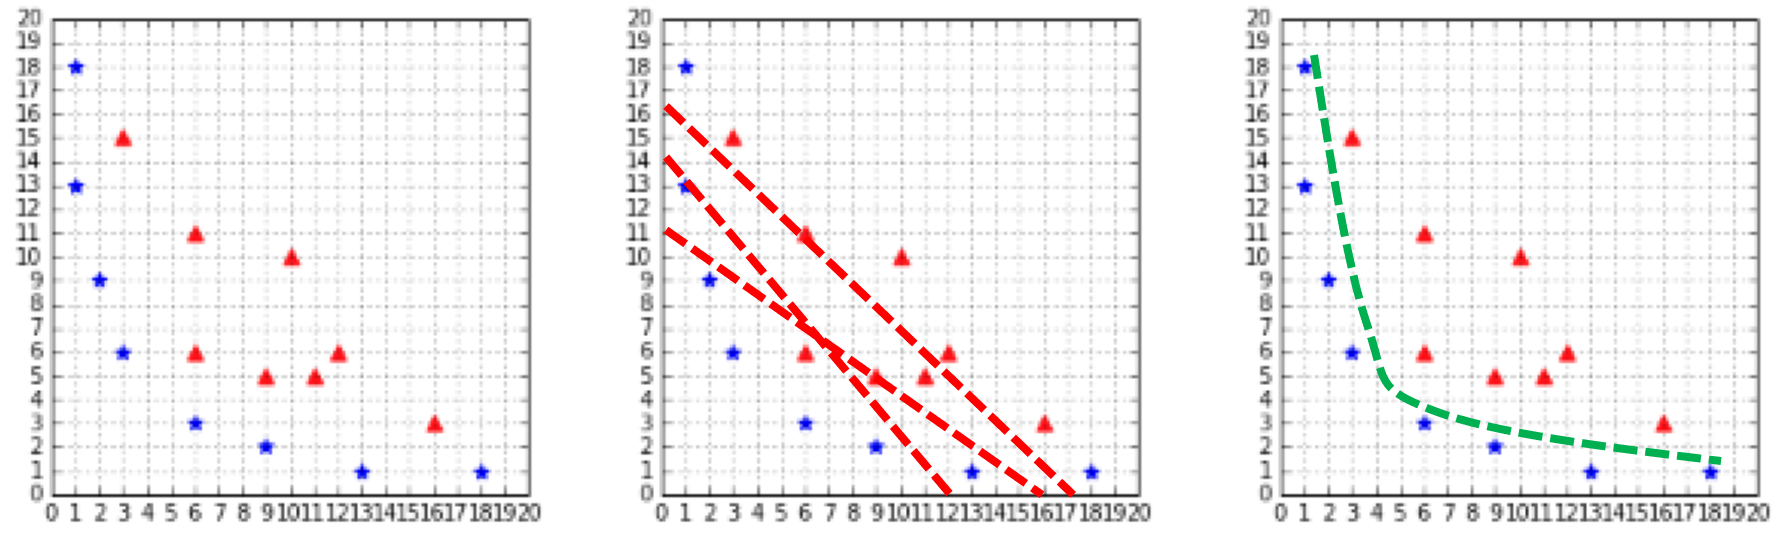
\includegraphics[width=0.58\textwidth]{assets/svm/nl__example.png}
    \subcaption{Non-linear decision boundary}
  \end{subfigure}

  \vspace*{0.3cm}

  
  \begin{subfigure}{\textwidth}
    \centering
    \begin{subfigure}{0.9\textwidth}
      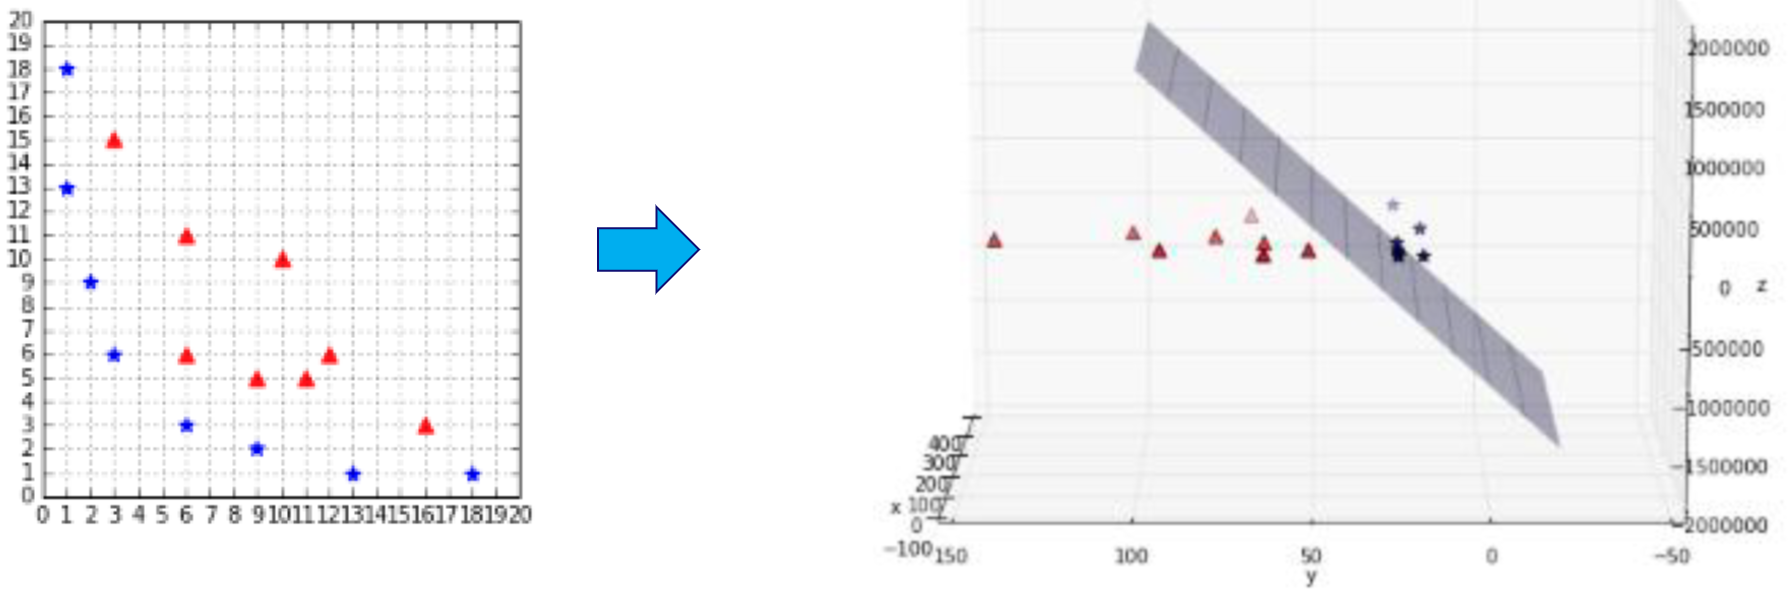
\includegraphics[width=0.64\textwidth]{assets/svm/nl__lift_1.png}\hspace*{0.3cm}
      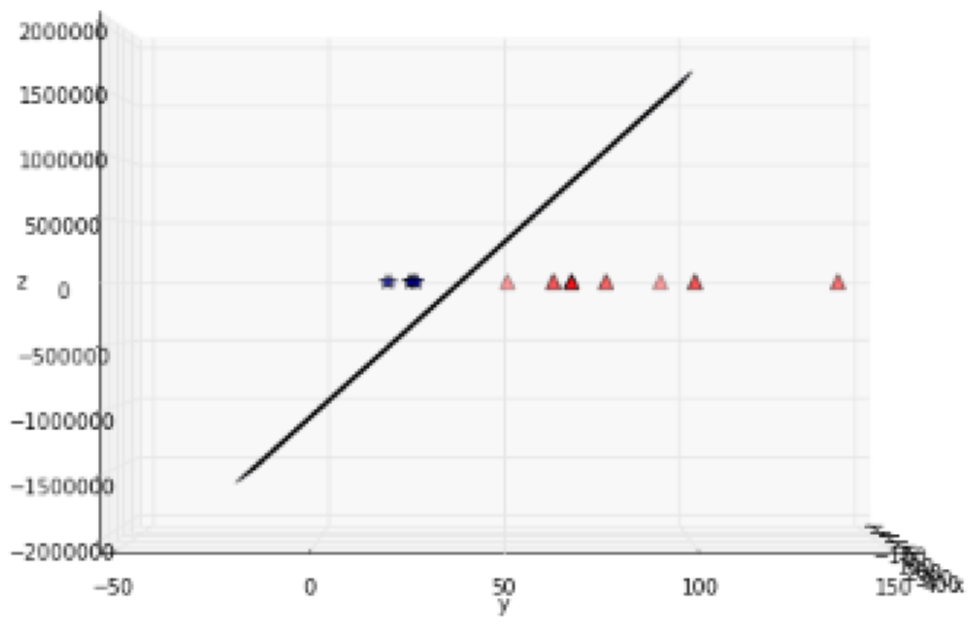
\includegraphics[width=0.32\textwidth]{assets/svm/nl__lift_2.png}
    \end{subfigure}
    \subcaption{Lift from $n=2$ to $n=3$}
  \end{subfigure}
  \caption{Non-linear separation}
  \label{fig:5_not_linear_separable}
\end{figure}

The mapping to lift the dimensions is similar to the one introduced for regression. So, we have the updated problem formulation:
\begin{align*}\begin{aligned}
  \text{Given a set of } m \text{ instances }& \big\{ (\cv{x}_i, y_i) \in \mathbb{R}^n\times\{-1,1\} \,\big|\, 1\leq i\leq m \big\}\sidenote{Soft-margin, dimension-lifted SVM problem}\\
  \text{Find a mapping }& {\color{burntorange} \phi\in\mathbb{R}^n \rightarrow \mathbb{R}^q }\text{ with } q>n\\
  &\begin{note}\text{\color{gray}E.g.: } \phi_0(x) = 1, \phi_1(x) = x, \phi_2(x) = x^2, \dots\end{note}\\
  \min_{\cv{w}, b, \epsilon}\frac{1}{2}\norm{\cv{w}}^2 +\, C\sum_{i=1}^m\epsilon_i \text{ s.t. } &\forall i: y_i(\cv{w}\cdot{\color{burntorange}\phi(\cv{x}_i)} + b) \geq 1 -\epsilon_i \begin{note}\text{ \color{gray}where }\epsilon_i\geq0\end{note}
\end{aligned}\end{align*}

For our example \ref{fig:5_not_linear_separable}, the mapping function was formulated as:
\begin{align*}
  \phi\in \ & \mathbb{R}^2 \rightarrow \mathbb{R}^3\\
  \phi(x_1, x_2)=\ &\left(x_1^2, \sqrt{2}x_1x_2, x_2^2\right)
\end{align*}

